\documentclass[prl,twocolumn,amsmath,amssymb,superscriptaddress]{revtex4-2}

% You may use additional packages as you see fit
\usepackage{graphicx}
\usepackage{verbatim}
\usepackage{braket}
\usepackage{epsfig}
\usepackage{epstopdf}
\usepackage{amsfonts}
\usepackage{amsthm}
\usepackage{float}
\usepackage{amsmath}
\usepackage{amssymb}
\usepackage{color}
\usepackage[usenames,dvipsnames,svgnames,table]{xcolor}
\usepackage{dsfont}
\usepackage{color}
\usepackage{grffile}
\usepackage{bm}

% ones I added
\usepackage{hyperref}
\usepackage{multirow}
\hypersetup{colorlinks=true,linkcolor=NavyBlue,citecolor=BrickRed,urlcolor=NavyBlue}

%end of packages

\begin{document}

\title{Biology Enzyme Lab Report}
\author{Luyu W.V.K.}
\date{\today}

\begin{abstract}
    Enzyme and substrate concentration are variables that both influence the rate of enzymatic reactions. In this case, we investigate the relationship by changing the concentration of our enzyme (Catalase) and keeping our substrate concentration ($H_{2}O_2$) constant.
\end{abstract}
\maketitle

\section{Introduction}
\section{Results}

Due to the time constraints, there were significant limitations to the data collected. Most noticeably, we only managed 2 replicates of each trial ($N=2$).

However, despite the low confidence due to lack of replicates, a general trend is still observable in our data. By processing our data with NumPy's array programming, we can visualize it using MatplotLib.

In Fig. \ref{fig:Volume}, we show the raw data (scattered points), trendlines ($2^{nd}$ degree polynomial fits), and averaged rates.

\begin{figure}[htb]
    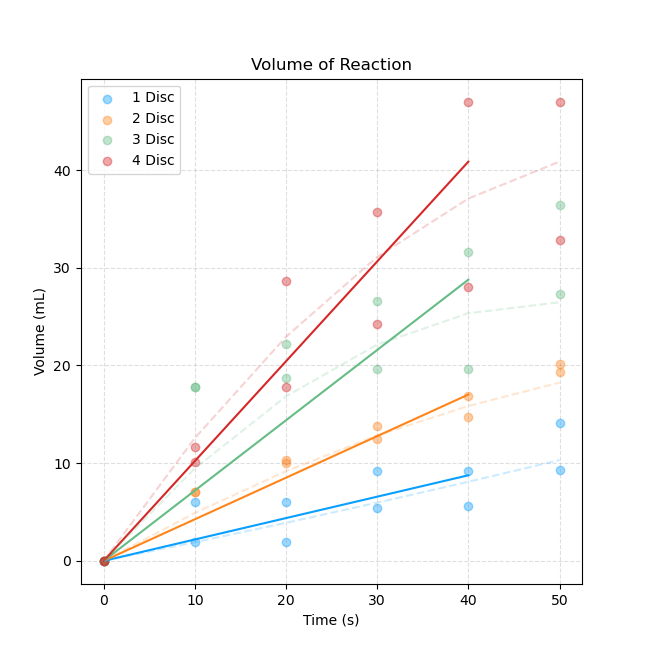
\includegraphics[width=1\linewidth]{Volume.png}
    \caption{\textbf{Graph of eudiometer volume vs. time}. Raw data points are shown as scattered points. The trendlines, visualized as dotted curves, are calculated with a $2^{nd}$ degree polynomial fit with a forced intercept. Lastly, the rate slopes (shown as solid lines) were calculated by averaging the slope of the LoBF for each trial's separate replicates.}
    \label{fig:Volume}
\end{figure}

Fig. \ref{fig:Volume} shows a visible upward trend in rate (slope of lines) as enzyme concentration is increased.

High levels of disparity between replicates of trials is visible in this graph, especially in trials with higher Catalase concentrations. Causes for this will be discussed in the errors section.



\begin{figure}[htb]
    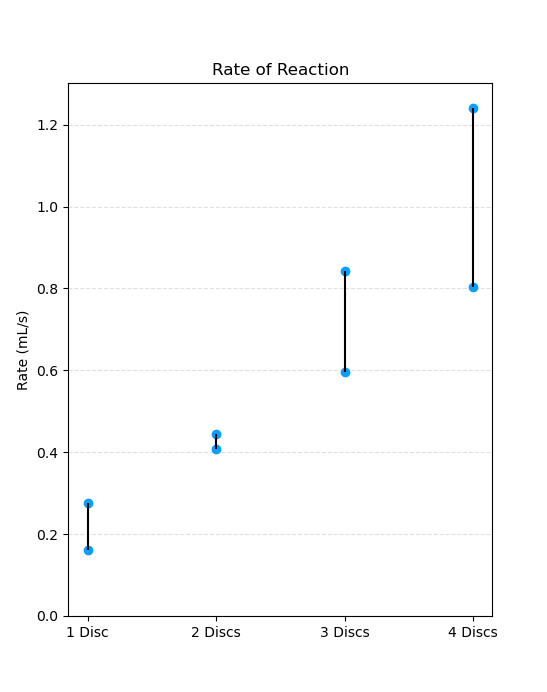
\includegraphics[width=1\linewidth]{Rate.png}
    \caption{\textbf{Graph of the reaction rate vs. enzyme concentration}. Each data point on the graph represents a replicate of a trial. The rate was found by calculating the slope of the LoBF for data ranging from 0-40s.}
    \label{fig:Rate}
\end{figure}

\newpage
Analyzing Fig. \ref{fig:Rate}, we see that our qualitative observation of increasing rate across trials in Fig. \ref{fig:Volume} is valid.

If we  take the average of replicate data points for each trial, a roughly linear trend can be seen between enzyme concentration and rate of reaction. This conforms with my hypothesis regarding the relationship between enzyme concentration and rate of reaction.

\newpage
\section{Errors}

There were numerous causes of error in our experiment, many of which were inherent to the equipment and methods used (non-human).
The most major errors of this variety were the following:

\begin{enumerate}
  \item \textbf{Large air bubbles in experiment caused massive granularity in measurements}. The $O_2$ gas produced by the reaction escaped the culture flask at irregular intervals (often greater than the sampling rate of 10s) and volumes (typically between 1-10mL). The effect of this phenomenon was that the measurements could not feasibly characterize the rate of reaction (which is continuous) correctly. To some level, this is hidden in the results by using best-fit lines, but it still heavily damages the accuracy and reproducibility of our results.
  \item \textbf{Variations in enzyme amount between discs made enzyme concentration uncontrollable}. A portion of the large disparity between replicates of each trial was likely caused by changes in enzyme concentration due to irregular amounts of catalase on each disc. While the purpose of the discs was to provide a quantized amount of enzyme on each packet, this was prone to error due to differing amounts of residue each disc left on the petri dish, changes in submersion time in the liver solution, and numerous other factors.
\end{enumerate}


\end{document}
